\documentclass[12pt,a4paper]{ctexart}

% ===========================================================================
% 页面设置
% ===========================================================================
\usepackage[top=2.5cm, bottom=2.5cm, left=3cm, right=3cm]{geometry}
\usepackage{graphicx}
\usepackage{float}
\usepackage{amsmath}
\usepackage{amssymb}
\usepackage{booktabs}
\usepackage{longtable}
\usepackage{hyperref}
\usepackage{caption}
\usepackage{subcaption}
\usepackage{enumitem}
\usepackage{fancyhdr}
\usepackage{tikz}
\usetikzlibrary{arrows,shapes,positioning,fit,backgrounds,calc}
\usetikzlibrary{shapes.geometric, arrows.meta, positioning, calc}
\usepackage{multirow}
\usepackage{array}
\usepackage{xcolor}
\usepackage{listings}

% ===========================================================================
% 代码块样式（仅用于附录）
% ===========================================================================
\lstset{
    basicstyle=\small\ttfamily,
    breaklines=true,
    frame=single,
    numbers=left,
    numberstyle=\tiny,
    commentstyle=\color{gray},
    keywordstyle=\color{blue},
    stringstyle=\color{red},
    captionpos=b,
    tabsize=4,
    language=Verilog
}

% ===========================================================================
% 页眉页脚
% ===========================================================================
\pagestyle{fancy}
\fancyhf{}
\fancyhead[L]{\small 数字系统课程设计}
\fancyhead[R]{\small 智能陪伴小车}
\fancyfoot[C]{\thepage}
\renewcommand{\headrulewidth}{0.4pt}

% ===========================================================================
% 文档标题
% ===========================================================================
\title{\Huge \textbf{课程设计报告}}
\author{}
\date{}
\begin{document}

% ===========================================================================
% 封面（在此修改课程信息）
% ===========================================================================
\begin{titlepage}
\thispagestyle{empty}
\begin{center}

\vspace*{2cm}

% 校徽（如需更换校徽，替换 images/school_logo.png）

\includegraphics[width=11cm]{images/school_logo.png}

\vspace{2cm}

{\Huge \textbf{课程设计报告}}

\vspace{2.5cm}

\begin{Large}
\begin{tabular}{rl}
\textbf{课程名称：}      & \underline{\makebox[7cm]{数字系统}} \\[1cm]
\textbf{任课老师：}      & \underline{\makebox[7cm]{李宇波}} \\[1cm]
\textbf{课程设计名称：}  & \underline{\makebox[7cm]{智能陪伴小车}} \\[1cm]
\textbf{完成日期：}      & \underline{\makebox[7cm]{2026年6月29日}} \\[1cm]
\textbf{小组：}          & \underline{\makebox[7cm]{第 3 小组}} \\[1cm]
\textbf{小组成员：}      & \underline{\makebox[7cm]{刘卓彦、郑一韬、李彦萱}} \\
\end{tabular}
\end{Large}

\vfill

\end{center}
\end{titlepage}

% ===========================================================================
% 目录
% ===========================================================================
\tableofcontents
\newpage

% ###########################################################################
% 第一节：目的和要求
% ###########################################################################
\section{项目的目的和要求}

\subsection{项目目的}
在智慧校园的建设从“基础设施数字化”向“以人为本的智能化”转型的背景下，学生心理健康日益受到重视。传统的心理咨询存在门槛高、非实时等问题。一款能够部署在宿舍、图书馆或心理咨询室的“智能陪伴小车”，能通过低成本、高效率的方式提供情感慰藉与日常交互，成为校园智慧生态中温情的一环。

本课程设计旨在设计并实现一台基于 FPGA 驱动的智能陪伴小车，通过Verilog完成全部控制逻辑，在FPGA上实现"传感器数据采集→控制算法运算→执行器驱动→人机交互"的完整闭环。我们设计的小车具备以下四项能力：

\begin{enumerate}[label=(\arabic*)]
    \item \textbf{自动跟随}：通过双路HC-SR04超声测距模块实时检测前方目标距离，利用双环PID控制器实现对人的自动跟随。
    \item \textbf{语音对话}：我们的小车能够通过麦克风模块接收用户指令，并根据不同情感进行回应，实现简单的问答交互。
    \item \textbf{多种行为}：智能陪伴小车能够根据场景和情感判断完成跟随、转弯、停止、自动跟随、前进与后退连接、原地旋转等4种主要运行模式之下多样的行为，通过对话返回的情感判断进行模式切换。
    \item \textbf{情感交互}：我们采用SSD1306 OLED显示屏（128$\times$64，I2C接口），根据当前工作模式实时显示不同的面部表情（开心/平静/伤心）。
    \item \textbf{电机驱动控制}：输出PWM信号及IN1/IN2方向信号，使用L298N电机驱动模块，驱动双路直流减速电机。
\end{enumerate}

\subsection{项目实现要求}

\begin{enumerate}[label=(\arabic*)]
    \item 综合利用数字系统课程相关知识，充分掌握并运用课内所学的Verilog语言、时序逻辑、模块化设计等知识和技能。
    \item 智能陪伴小车功能要主要采用Verilog语言实现，利用EGO1开发板运行。
    \item 各模块之间接口清晰、职责分明，便于独立仿真调试与系统联调。
    \item 超声波测距刷新周期约为$50\text{ ms}$，采用双环PID算法，期望静态跟随距离稳定在约$50\text{ cm}$，转向环能根据左右距离差实时调整。
    \item OLED显示需支持模式切换时的自动复位和表情切换。
    \item 各模块之间电压转换需符合各器件的工作电压要求。
\end{enumerate}

% ###########################################################################
% 第二节：原理
% ###########################################################################
\section{原理与设计}
\subsection{外观设计}
我们基于功能实现要求设计了三层小车，除了基本车架之外，电子元器件包含SSD1306 OLED显示屏、HC-SR04超声测距模块、电压转换器、L298N电机驱动模块、直流减速电机、麦克风模块、EGO1 FPGA开发板、ASRPRO语音识别芯片以及电源模块。小车外观设计如下图所示：
\begin{figure}[H] 
    \centering % 使图片居中对齐
    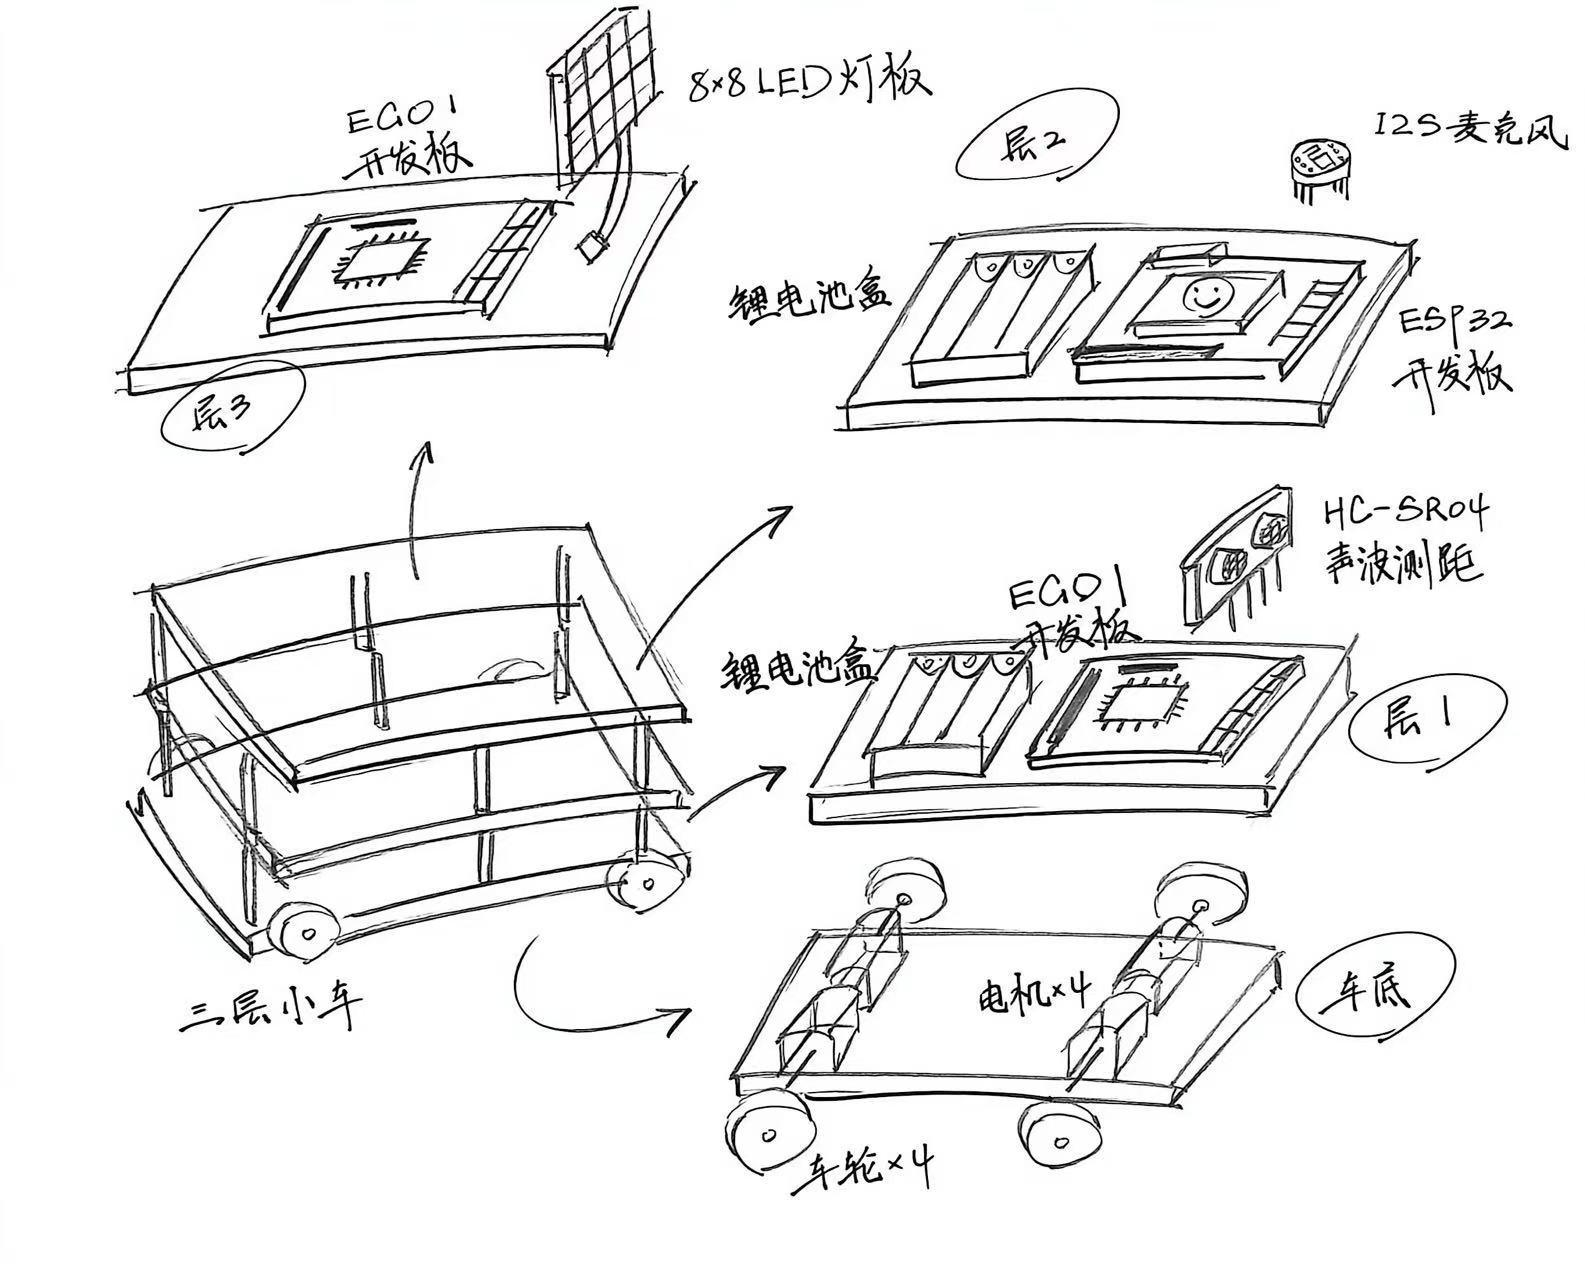
\includegraphics[width=0.8\textwidth]{images/小车设计.jpeg} 
    \caption{外观设计图} 
    \label{fig:外观设计}
\end{figure}

\subsection{系统总体架构}

我们在项目的代码设计中采用模块化设计，整体架构如下图所示。智能陪伴小车由运控系统、OLED 显示系统、语音交互系统组成。

\begin{figure}[H]
\centering
\begin{tikzpicture}[
    auto,
    node distance = 1.2cm and 1.5cm,
    box/.style = {rectangle, draw=black, thick, fill=white, minimum width=3.5cm, minimum height=1cm, align=center, font=\small},
    container/.style = {rectangle, draw=blue!70!black, dashed, thick, fill=blue!5, inner sep=0.5cm, font=\small\bfseries}
]
    % 1. ASRPRO Node
    \node [box, fill=gray!10] (asr) {ASRPRO语音识别模块};

    % 2. FPGA Container (Placeholder for positioning, drawn later)
    \node [box, below=1.8cm of asr, xshift=-2.5cm] (top) {运控模块};
    \node [box, right=2.5cm of top] (oled_sub) {OLED表情控制(I2C 协议)};
    \node [box, below=1.5cm of top] (car) {运控模块};

    % 3. External Peripherals Nodes
    \node [box, right=2.5cm of car] (oled_screen) {OLED显示屏};
    \node [box, below=1.5cm of car] (motor) {L298N驱动模块+直流电机};

    % 4. Draw FPGA Container Box based on inner nodes
    \begin{scope}[on background layer]
        \node [container, fit=(top) (oled_sub) (car), label={[anchor=north west]north west:EGO1开发板}] (fpga) {};
    \end{scope}

    % 5. Interconnections (Arrows)
    % ASRPRO to FPGA Top
    \draw [-{Stealth[scale=1.2]}, thick] (asr.south) -- node[left, align=center, font=\footnotesize] {2-bit 情绪代码} ($(top.north)+(0,0.5cm)$) -- (top.north);
    
    % Top to OLED Sub
    \draw [-{Stealth[scale=1.2]}, thick] (top.east) -- node[above, font=\footnotesize] {情绪标签} (oled_sub.west);
    
    % Top to Car Follow
    \draw [-{Stealth[scale=1.2]}, thick] (top.south) -- (car.north);
    
    % OLED Sub to OLED Screen
    \draw [-{Stealth[scale=1.2]}, thick] (oled_sub.south) -- node[right, font=\footnotesize] {I2C总线} (oled_screen.north);
    
    % Car Follow to Motor
    \draw [-{Stealth[scale=1.2]}, thick] (car.south) -- node[right, font=\footnotesize] {PWM信号} (motor.north);
\end{tikzpicture}
\caption{基于FPGA的智能陪伴小车异构控制系统总体架构图}
\label{fig:system_architecture}
\end{figure}

\subsection{PID控制原理}

\subsubsection{算法原理}

我们的智能陪伴小车在运动控制模块设计时采用PID控制算法，其数学表达为：
\begin{equation}
u(t) = K_p \, e(t) + K_i \int_0^t e(\tau) \, d\tau + K_d \, \frac{de(t)}{dt}
\label{eq:pid_continuous}
\end{equation}

其中$e(t)$为偏差信号，$K_p$、$K_i$、$K_d$分别为比例、积分、微分系数。由于FPGA是离散数字系统，式~\ref{eq:pid_continuous}需离散化后在硬件中实现。我们在算法设计时采用定点数运算以节省硬件资源，即内部计算精度保留8位小数位，输出时通过右移8位恢复实际量纲：

\begin{align}
e_k &= \text{target} - \text{actual} \nonumber\\
P_k &= K_p \cdot e_k \nonumber\\
I_k &= I_{k-1} + e_k \nonumber\\
D_k &= K_d \cdot (e_k - e_{k-1}) \nonumber\\
u_k &= \frac{P_k + K_i \cdot I_k + D_k}{256} \label{eq:pid_discrete}
\end{align}

\subsubsection{双环 PID 结构}

为实现小车对人的平滑跟随，我们在设计中采用双环PID结构。

\textbf{速度环}：以50cm对应的超声波计数值为目标值，以两路超声波平均距离计数值为反馈量，输出基础速度信号$v_{\text{speed}}$。当小车距离目标过远时加速接近，过近时减速甚至后退。

\textbf{转向环}：以0为目标值（代表左右距离相等），以两路超声波距离差为反馈量，输出转向修正信号$v_{\text{turn}}$。当目标偏左时，右轮加速、左轮减速/反转，使小车向右修正方向。

理论上，两环输出经\textbf{差速混控公式}合成左右轮占空比：
\begin{equation}
\begin{cases}
\text{left\_duty} = \text{speed\_ctrl} + \text{turn\_ctrl} \\[4pt]
\text{right\_duty} = \text{speed\_ctrl} - \text{turn\_ctrl}
\end{cases}
\label{eq:mixing}
\end{equation}

这种差速驱动方式使得转向修正不影响整体前进速度，保证了跟随过程的平顺性。两个PID控制器实例的参数配置如表~\ref{tab:pid_params} 所示。速度环的比例系数和积分系数均高于转向环，这是因为距离跟随对响应速度要求更高，而转向修正需要更保守的参数以避免方向振荡。

\begin{table}[H]
\centering
\caption{PID 控制器实例化参数}
\label{tab:pid_params}
\begin{tabular}{cccccc}
\toprule
\textbf{实例} & \textbf{用途} & \textbf{$K_p$} & \textbf{$K_i$} & \textbf{$K_d$} & \textbf{输出范围} \\
\midrule
u\_speed\_pid & 速度控制 & 512 & 128 & 256 & $\pm$200 \\
u\_turn\_pid  & 转向控制 & 384 & 64  & 192 & $\pm$150 \\
\bottomrule
\end{tabular}
\end{table}

\subsection{超声波测距原理}

\subsubsection{HC-SR04 传感器工作原理}

HC-SR04是一种常用的非接触式距离测量模块，工作频率为40kHz，测距范围为2cm-400cm（但是在实际应用中没有那么大）。其工作流程如下：

\begin{enumerate}[label=(\arabic*)]
    \item 主控器向Trig引脚发送一个时长$\ge 10\,\mu$s的高电平触发脉冲。
    \item 模块内部自动发出8个40kHz的超声波脉冲，同时将Echo引脚拉高。
    \item 超声波在空气中传播，遇到障碍物后反射回来。
    \item 模块接收到回波后将Echo引脚拉低。
    \item 主控器通过测量Echo高电平的持续时间$t_{\text{echo}}$来计算距离：
    \begin{equation}
    d = \frac{v_{\text{声}} \cdot t_{\text{echo}}}{2}
    \label{eq:distance}
    \end{equation}
\end{enumerate}

\subsubsection{双路交替测距设计}
为实现对目标方位的感知，我们在小车头部左右各安装一个HC-SR04超声波传感器。FPGA通过FSM交替触发和测量两路传感器：
\begin{center}
\textsf{IDLE $\to$ TRIG\_LEFT $\to$ WAIT\_ECHO\_L $\to$ MEASURE\_L $\to$ STORE\_L} \\
\textsf{$\to$ TRIG\_RIGHT $\to$ WAIT\_ECHO\_R $\to$ MEASURE\_R $\to$ STORE\_R} \\
\textsf{$\to$ WAIT\_50MS $\to$ IDLE（循环）}
\end{center}

关键设计要点：
\begin{itemize}
    \item \textbf{触发脉冲宽度}：1000个时钟周期为10 $\mu$s，满足HC-SR04对触发脉宽的最低要求。
    \item \textbf{超时保护}：等待回波和测量阶段均设置 3,000,000 个时钟周期（约30 ms）的超时上限。若Echo信号在此时间内未出现或未结束，状态机自动跳转到下一阶段，避免因传感器故障导致系统死锁。
    \item \textbf{异步信号同步}：Echo信号为异步输入，通过两级寄存器同步消除亚稳态，再通过边沿检测电路捕获上升沿和下降沿。
    \item \textbf{测量周期}：完整一轮左右交替测距约需50ms，对应于20 Hz的控制更新频率。对于步行速度的跟随场景，该更新率满足实时性要求。
\end{itemize}

测距完成后计算两个关键信号供PID控制器使用：
\begin{align}
\text{avg\_cnt} &= (\text{left\_cnt} + \text{right\_cnt}) \gg 2 \quad \text{（平均距离计数值）} \label{eq:avg}\\
\text{diff\_signed} &= \text{right\_cnt} - \text{left\_cnt} \quad \text{（左右距离差）} \label{eq:diff}
\end{align}

\subsection{PWM 电机驱动原理}

\subsubsection{H 桥驱动与 PWM 调速}

在制作智能陪伴小车时，我们采用了L298N双路H桥电机驱动模块控制两个直流减速电机。H桥电路通过四个开关管的通断组合实现电机的正转、反转和制动。L298N的每路H桥需要三个控制信号：ENA和两个方向输入端（IN1、IN2）。

理论上脉宽调制可以通过调节单位时间内占空比来控制电机的平均电压，从而调节转速。PWM参数设计如下：
\begin{itemize}
    \item \textbf{载波频率}：20kHz（$\frac{100\,\text{MHz}}{5000} = 20\,\text{kHz}$。
    \item \textbf{占空比分辨率}：8 位（0-255），经限幅后映射到PWM比较值为0-4999。
    \item \textbf{计数范围}：0-4999，每个PWM周期将计数器值与占空比比较值比较，生成PWM波形。
\end{itemize}
但是在实际的应用中，我们因为电压转换器不足没有采用占空比，利用正转和反转来实现转弯、转圈等功能。

\subsubsection{方向控制逻辑}

电机方向由 IN1/IN2 信号的组合控制，逻辑如表~\ref{tab:motor_logic} 所示。该逻辑将 PID 输出的有符号控制量直接映射为电机方向和转速：正duty值对应正转，负duty值对应反转，零值对应停止。

\begin{table}[H]
\centering
\caption{电机方向控制逻辑（适配 L298N）}
\label{tab:motor_logic}
\begin{tabular}{cccc}
\toprule
\textbf{duty 符号} & \textbf{IN1} & \textbf{IN2} & \textbf{电机状态} \\
\midrule
duty $>$ 0  & 1 & 0 & 正转（前进） \\
duty $<$ 0  & 0 & 1 & 反转（后退） \\
duty $=$ 0  & 0 & 0 & 停止（刹车） \\
\bottomrule
\end{tabular}
\end{table}

\subsection{OLED显示与I2C通信原理}

\subsubsection{SSD1306 OLED显示屏}

为了更好显示表情我们选用1.3寸SSD1306 OLED 显示屏，通过I2C串行总线与FPGA通信。SSD1306内部集成GDDRAM，按页组织——共8页、每页128列$\times$8位。写入GDDRAM的数据直接映射到屏幕像素（1=点亮，0=熄灭）。

\subsubsection{I2C 通信协议}

I2C是一种双线串行总线协议，仅需SCL和SDA两条信号线。在小车设计中，FPGA作为I2C主机，OLED作为从机，实现了一个完整的I2C Master控制器，特性如下：

\begin{itemize}
    \item \textbf{SCL 频率}：约200kHz，满足SSD1306 标准模式和快速模式的要求。
    \item \textbf{协议完整性}：自动生成START和STOP条件，每字节传输后检测从机ACK/NACK应答。
    \item \textbf{SDA 双向控制}：通过三态门实现SDA的输入/输出切换，在ACK检测阶段释放总线由从机驱动。
    \item \textbf{错误处理}：从机未应答时输出Error信号，供上层模块处理。
\end{itemize}
I2C Master状态机共约58个状态，完整覆盖一次写操作流程：START $\to$ 发送从机地址（7bit+W）$\to$ ACK $\to$ 发送寄存器地址（8bit）$\to$ ACK $\to$ 发送数据（8bit）$\to$ ACK $\to$ STOP。

\subsection{情感化表情显示设计}

\begin{figure}[H]
\centering
\begin{tikzpicture}[
    box/.style={rectangle, draw, minimum width=2cm, minimum height=1.2cm, align=center, font=\small},
    arrow/.style={->, >=stealth, thick}
]

\node[box, fill=green!10] (sw) {状态输入};
\node[box, right=1.8cm of sw, fill=blue!10] (detect) {模式检测};
\node[box, right=1.8cm of detect, fill=yellow!10] (select) {字模选择};
\node[box, right=1.8cm of select, fill=red!10] (render) {渲染输出};
\node[box, right=1.8cm of render, fill=gray!10] (screen) {OLED 屏幕};

\draw[arrow] (sw) -- (detect) node[midway, above] {\footnotesize 模式值};
\draw[arrow] (detect) -- (select) node[midway, above] {\footnotesize 复位+选择};
\draw[arrow] (select) -- (render) node[midway, above] {\footnotesize 32B点阵};
\draw[arrow] (render) -- (screen) node[midway, above] {\footnotesize I2C写入};

\end{tikzpicture}
\caption{情感化表情显示的信号通路}
\label{fig:emotion_path}
\end{figure}

情感交互是我们的一个创新点，表情切换的信号通路如图~\ref{fig:emotion_path} 所示：语音交互后判断情感状态 →检测变化并复位OLED→根据sw值选择开心/平静/难过对应的字模数据组→将字模转换为I2C写命令序列 →经FPGA发送到OLED屏幕。每套表情由我们自定义的点阵字符拼接而成，共同构建一张完整的表情画面。

\subsection{多模式行为切换设计}
\begin{figure}[H] 
    \centering % 使图片居中对齐
    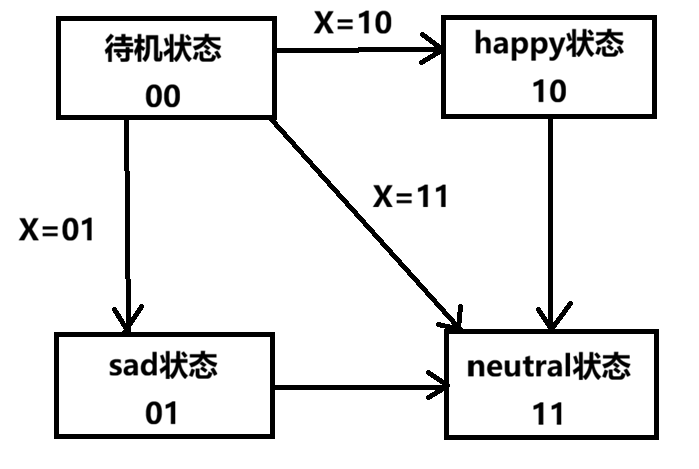
\includegraphics[width=0.6\textwidth]{images/状态转换.png} 
    \caption{状态转换图} 
    \label{fig:状态转换}
\end{figure}

系统的4种工作模式及对应行为如表~\ref{tab:modes} 所示。其中FOLLOW为常态运行模式；STOP、FWD\_REV和SPIN为情感动作，执行完预定义动作序列后自动返回FOLLOW。这一设计确保小车不会长时间停留在非跟随状态。

\begin{table}[H]
\centering
\caption{小车 4 种运行模式定义}
\label{tab:modes}
\begin{tabular}{cclcl}
\toprule
\textbf{mode[1:0]} & \textbf{模式名称} & \textbf{行为描述} & \textbf{持续时间} & \textbf{OLED 表情} \\
\midrule
00 & STOP      & 电机静止，PWM 输出置零          & 稳态 & --- \\
01 & FOLLOW    & PID自动跟随目标                & 平静             & 正常 \\
10 & FWD\_REV  & 前进2s与后退2s交替 & 共约8s & 难过 \\
11 & SPIN      & 左轮正转+右轮反转& 10s   & 开心 \\
\bottomrule
\end{tabular}
\end{table}

模式切换由car\_follow模块内部的action\_busy标志位管理：当检测到模式切换边沿时，action\_busy 置位并锁定当前动作直至执行完毕，期间新的模式切换请求被忽略。这一互锁机制有效防止了用户在动作执行中切换模式导致的控制信号冲突。

\subsection{语音识别与跨芯片异步通信}
我们在设计语音模块时先后采用两种方案：分别为基于LLM的多模态情感映射与本地化边缘语音芯片ASRPRO。但是由于麦克风硬件识别准确率不高，尽管我们成功实现了调用大模型并结合输入语言返回恢复以及设定感情，我们最后还是采用了使用ASRPRO芯片的方案。
\begin{figure}[H]
\centering
\begin{tikzpicture}[
    auto,
    node distance = 1.0cm and 1.2cm,
    box/.style = {rectangle, draw=black, thick, fill=white, minimum width=3.2cm, minimum height=1cm, align=center, font=\small},
    container/.style = {rectangle, draw=#1, dashed, thick, fill=#1!5, inner sep=0.4cm, font=\small\bfseries}
]

    % 1. ASRPRO Subsystem Container
    \node [box, fill=gray!10] (asr_core) {命令词匹配};
    \node [box, fill=gray!10, right=1.5cm of asr_core] (asr_io) {GPIO引脚驱动};
    
    % 2. FPGA Inner Modules
    \node [box, below=3cm of asr_io, xshift=-1.3cm] (sync_reg) {异步信号同步器};
    \node [box, below=1cm of sync_reg] (top) {核心主控状态机};
    \node [box, right=1.7cm of top] (oled_sub) {OLED 表情控制系统};
    \node [box, below=1cm of top] (car) {运控模块};

    % 3. Peripherals
    \node [box, right=1.7cm of oled_sub] (oled_screen) {OLED 显示屏};
    \node [box, below=1cm of car] (motor) {L298N 驱动 + 电机};

    % 4. Containers
    \begin{scope}[on background layer]
        \node [container=orange!80!black, fit=(asr_core) (asr_io), label={[anchor=north west]north west:ASRPRO语音芯片}] (asr_box) {};
        \node [container=blue!70!black, fit=(sync_reg) (top) (oled_sub) (car), label={[anchor=north west]north west:FPGA}] (fpga_box) {};
    \end{scope}

    % 5. Connections
    % Inside ASRPRO
    \draw [-{Stealth[scale=1.0]}, thick] (asr_core) -- node[above, font=\footnotesize] {语义触发} (asr_io);
    
    % ASRPRO to FPGA
    \draw [-{Stealth[scale=1.2]}, thick, color=orange!80!black] (asr_io.south) -- node[right, font=\footnotesize, align=left] {硬件电平脉冲\\($t > 10\text{ ms}$)} (sync_reg.north);
    
    % FPGA Internal Flow
    \draw [-{Stealth[scale=1.0]}, thick] (sync_reg.south) -- node[left, font=\footnotesize] {2-bit mode编码} (top.north);
    \draw [-{Stealth[scale=1.0]}, thick] (top.east) -- node[above, font=\footnotesize] {情绪标签} (oled_sub.west);
    \draw [-{Stealth[scale=1.0]}, thick] (top.south) -- (car.north);
    
    % To External Peripherals
    \draw [-{Stealth[scale=1.2]}, thick] (oled_sub.east) -- node[above, font=\footnotesize] {I2C 总线} (oled_screen.west);
    \draw [-{Stealth[scale=1.2]}, thick] (car.south) -- node[right, font=\footnotesize] {PWM\&方向控制} (motor.north);

\end{tikzpicture}
\caption{包含语音识别交互与异步采样机制的系统总体架构原理图}
\label{fig:system_architecture_v2}
\end{figure}
下面主要对ASRPRO的原理与设计进行阐述：
\begin{itemize}
    \item \textbf{边缘语音识别与语义映射原理}：ASRPRO芯片内部集成了本地神经网络微型加速器，在经过特定唤醒词与命令词的固件烧录后，芯片可在本地完成对麦克风采集到的音频流的特征提取与匹配。当识别到有效语义后，芯片内部的MCU会将高级文本语义转换为特定引脚的电平跳变。
    \item \textbf{跨时钟域异步脉冲通信机制}：由于ASRPRO芯片内部核心时钟与FPGA主控系统时钟相互独立，为避免直接采用UART串口通信给FPGA状态机带来轮询开销与时序亚稳态风险，我们使用了电平脉冲宽度采样协议：ASRPRO 在识别到不同命令后，向 FPGA 的 GPIO 引脚发送特定时间窗口宽度的硬件电平脉冲。FPGA端的接收控制模块在主频下对该引脚实施持续的两级寄存器打拍同步，以消除亚稳态。同时，在脉冲有效期间进行计数采样。若电平宽度满足预设阈值，则将该状态锁存进一个2-bit的情绪代码寄存器，从而在极低硬件资源消耗下实现了高抗干扰性的跨芯片数据传递。
\end{itemize}

\begin{figure}[H] 
    \centering % 使图片居中对齐
    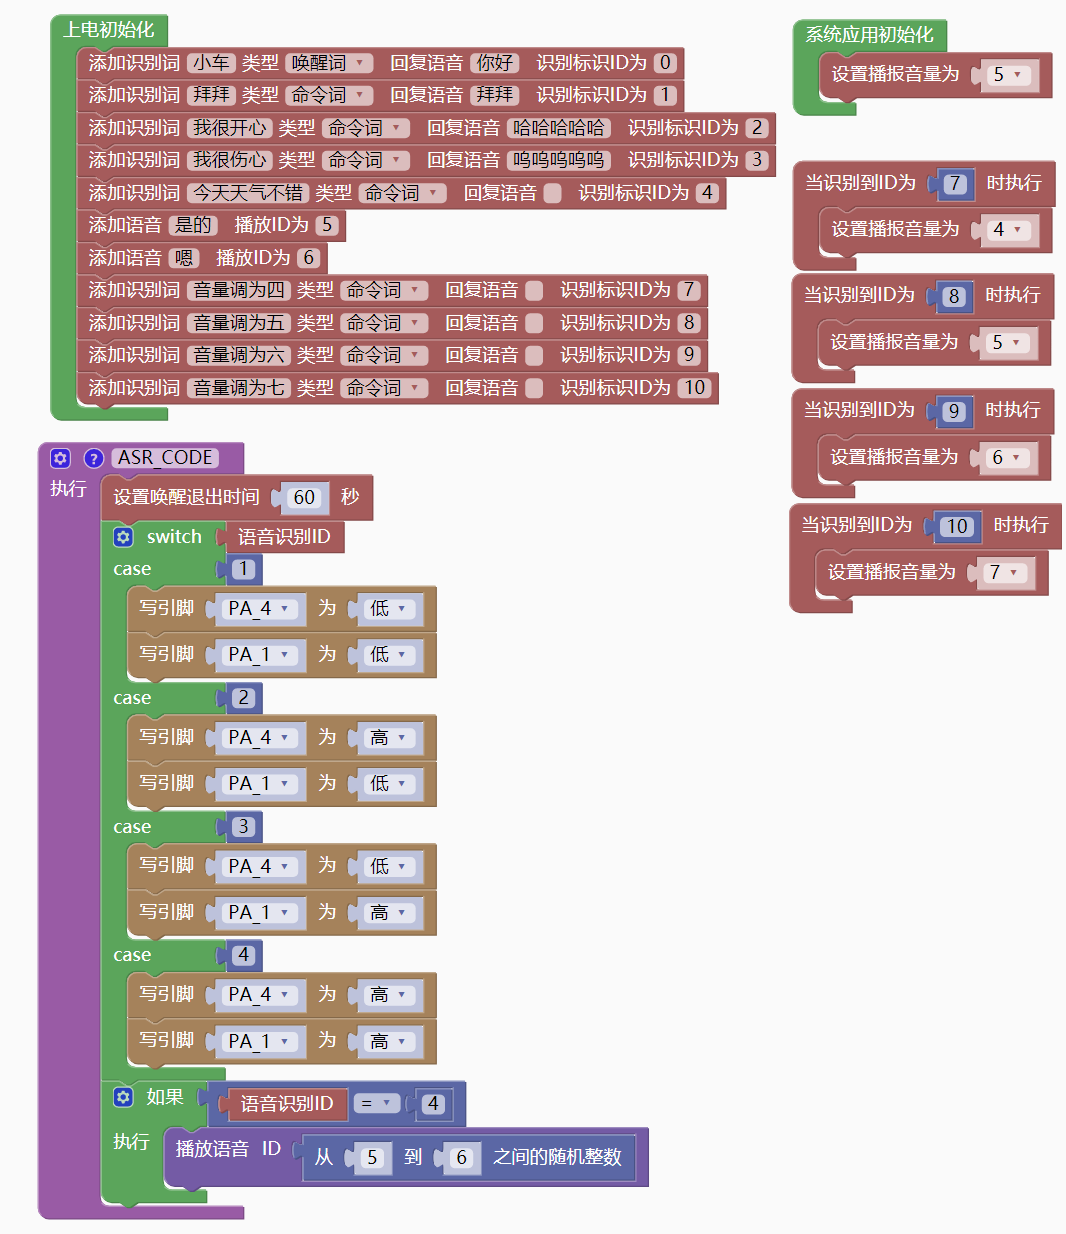
\includegraphics[width=0.8\textwidth]{images/语音模块代码.png} 
    \caption{语音模块代码} 
    \label{fig:语音模块代码}
\end{figure}

% ###########################################################################
% 第三节：结果和分析
% ###########################################################################
\section{测试和分析}

\subsection{自动跟随功能测试与分析}

在FOLLOW模式下对小车进行跟随性能测试。测试方法：以行人作为跟随目标，在小车前方以步行速度移动，观察小车跟随行为。

\textbf{测试结果：}

天崩开局，我们的小车因为电机驱动能力不足跑不动，只能把充电宝拿起来像遛电子宠物一样才行。开始人为遛之后继续天崩，这个小车在教学楼里乱跑，动不动就倒车，或者拐弯。经排查是因为超声波过于灵敏，但是到空旷的户外他又不太跑得动。只能找较为空的室内。最终在较理想的情况下，小车能实现即定功能。

尽管我们的双环PID结构在跟随场景中理论上控制效果非常好。但是因为硬件太差，优势被严重削弱。

\subsection{语音控制模式切换功能测试与分析}

我们将语音与运控进行联测，依次通过语音对话测试了FOLLOW $\to$ SPIN $\to$ FOLLOW $\to$ FWD\_REV $\to$ FOLLOW 的完整切换流程。

\textbf{测试结果：}
\begin{itemize}
    \item \textbf{SPIN模式}：切换到SPIN后，左轮正转、右轮反转，OLED同步切换为开心表情。大约10秒后自动回到 FOLLOW 模式。
    \item \textbf{FWD\_REV模式}：切换到FWD\_REV后，小车按"前进2s后退2s"的序列循环执行，OLED同步切换为难过表情。共约8秒后自动回到FOLLOW模式
    \item \textbf{实地测试}：我们遗憾的发现，我们的小车由于电机驱动能力太差，在摩擦较大的地面上无法完成任何运动，只有在非常光滑的地面上才能完成动作。同时，因为我们的电压转换器不够，无法实现PWM通过占空比调速，导致小车在执行转弯时只能依靠一轮往前一轮往后，不太灵敏。
\end{itemize}

对于此块的测试总体较为顺利，没有遇到大问题，毕竟代码运行没有任何问题，驱动能力太差我们也无法解决，或许换个更强力的电机效果会理想很多。

\subsection{OLED 显示功能测试与分析}

\textbf{测试结果：}
\begin{itemize}
    \item \textbf{上电初始化}：FPGA上电后，理想状态，OLED会完成SSD1306初始化序列并显示对应表情，但实际出现花屏，原因是有时候FPGA供电电压不稳定。
    \item \textbf{表情切换}：通过语音进行模式切换，理想状态OLED会在约100 ms内完成重新初始化及新表情显示。但是在实际的验证时多次出现了OLED表情没有切换，在每次排查时均发现信号输入正常。我们先尝试修改代码，使用寄存器保持信号的持续输入，但是不稳定状态没有很大改善，最后经过排查，我们认为是四脚oled硬件不稳定导致的。
\end{itemize}

OLED的不稳定是我们项目调试过程中的一大问题，我们先后尝试了多种方法，包括使用寄存器保持信号、提高I2C频率等，但仍然存在偶发的花屏或表情切换失败现象。最终我们认为问题主要出在OLED模块本身的硬件质量上，买硬件还是要买好一点的（小车也是这样）。

\subsection{实践过程中的优化}
\subsubsection{语音通信架构方案的迭代}
最初设计尝试利用ESP32模块连接Wi-Fi，通过云端调用大语言模型API 以及网络ASR/TTS实现远程智能对话。但是由于硬件问题放弃。

最后改为本地部署ASRPRO语音芯片。虽然牺牲了开放式对话能力，但换取了识别正确率与较快的响应速度。

\subsubsection{总线通信协议的精简}
原计划在ASRPRO与主控FPGA之间建立标准的UART串行异步收发总线。但是过于复杂，且在FPGA端需要轮询接收缓冲区，增加了设计复杂度和时序风险。

我们将其精简为引脚电平脉冲采样方案。FPGA仅需在特定时间窗口内对硬件引脚进行电平锁存即可，降低了数字逻辑的复杂度，提高了硬件抗干扰能力。同时我们也将最初设计的两块FPGA和一块ESP32精简为仅用两块FPGA驱动。


% ###########################################################################
% 第四节：成果
% ###########################################################################
\section{项目成果}

\subsection{实物总览}

经过设计、编码、仿真和上板调试，本小组成功实现了一台基于FPGA驱动的智能陪伴小车。小车的实物组成部分包括：

\begin{itemize}
    \item \textbf{FPGA开发板}：作为系统主控制器，搭载 100 MHz 板载晶振，提供全部数字逻辑资源。
    \item \textbf{双路HC-SR04 超声波传感器}：安装于小车前方左右两侧，实现目标方位感知。
    \item \textbf{双路直流减速电机+L298N驱动模块}：提供差速驱动能力，最高 PWM 载波频率 20 kHz。
    \item \textbf{SSD1306 OLED显示屏}：通过I2C总线与FPGA连接，实时显示情感表情。
    \item \textbf{电源模块}：由电池为电机驱动供电、搭载两个充电宝为FPGA和ASRPRO供电。
\end{itemize}
小车外观如下：
\begin{figure}[H] 
    \centering % 使图片居中对齐
    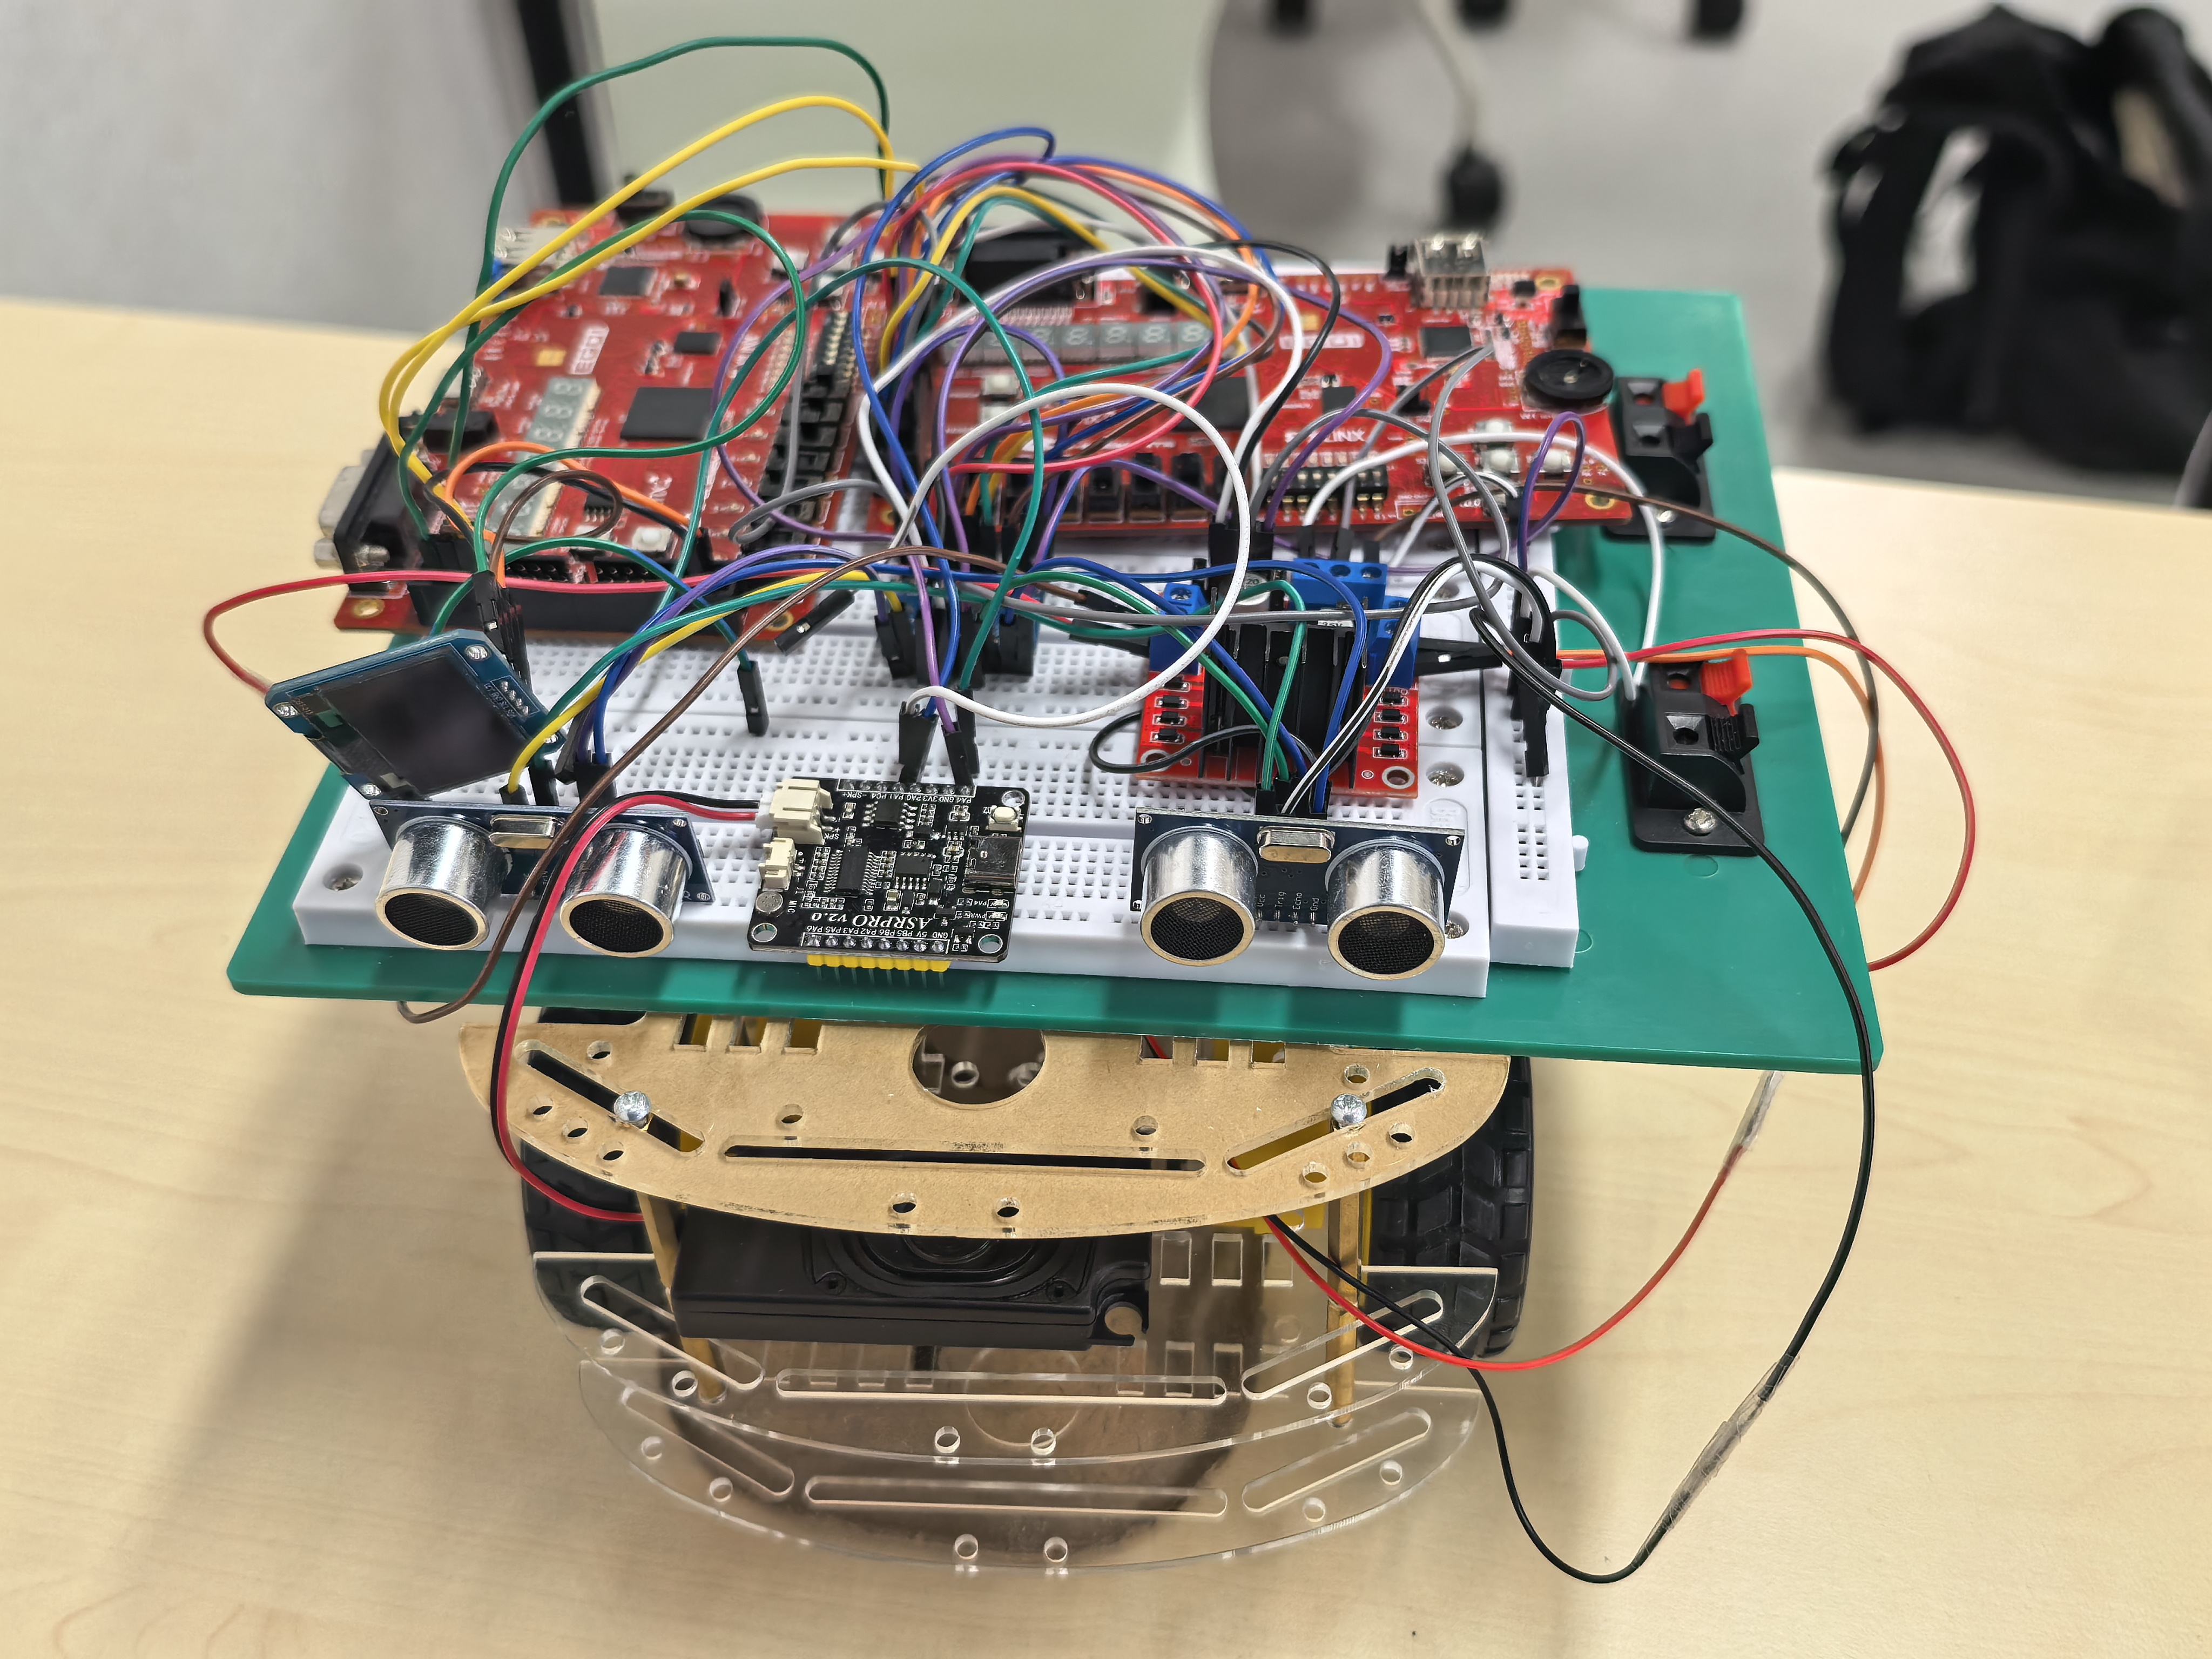
\includegraphics[width=0.8\textwidth]{images/小车外观.jpg} 
    \caption{小车外观} 
    \label{fig:外观}
\end{figure}

\subsection{实现的功能}

\begin{enumerate}[label=(\arabic*)]
    \item \textbf{智能跟随}：过测距传感器实时采集距离数据，FPGA快速处理传感信号，输出PWM控制信号调节电机转速，实现小车对目标对象的自动稳定跟随。
    \item \textbf{语音情感联动动作功能}：根据不同语音情感识别结果，FPGA控制小车执行差异化运动动作，实现情感与动作的精准联动，完成拟人化陪伴反馈。
    \item \textbf{OLED情感表情显示功能}：FPGA接收语音情感指令，驱动OLED显示屏实时显示对应情感表情（笑脸、平静脸、委屈脸），实现用户情感的可视化反馈。
\begin{figure}[H] 
    \centering % 使图片居中对齐
    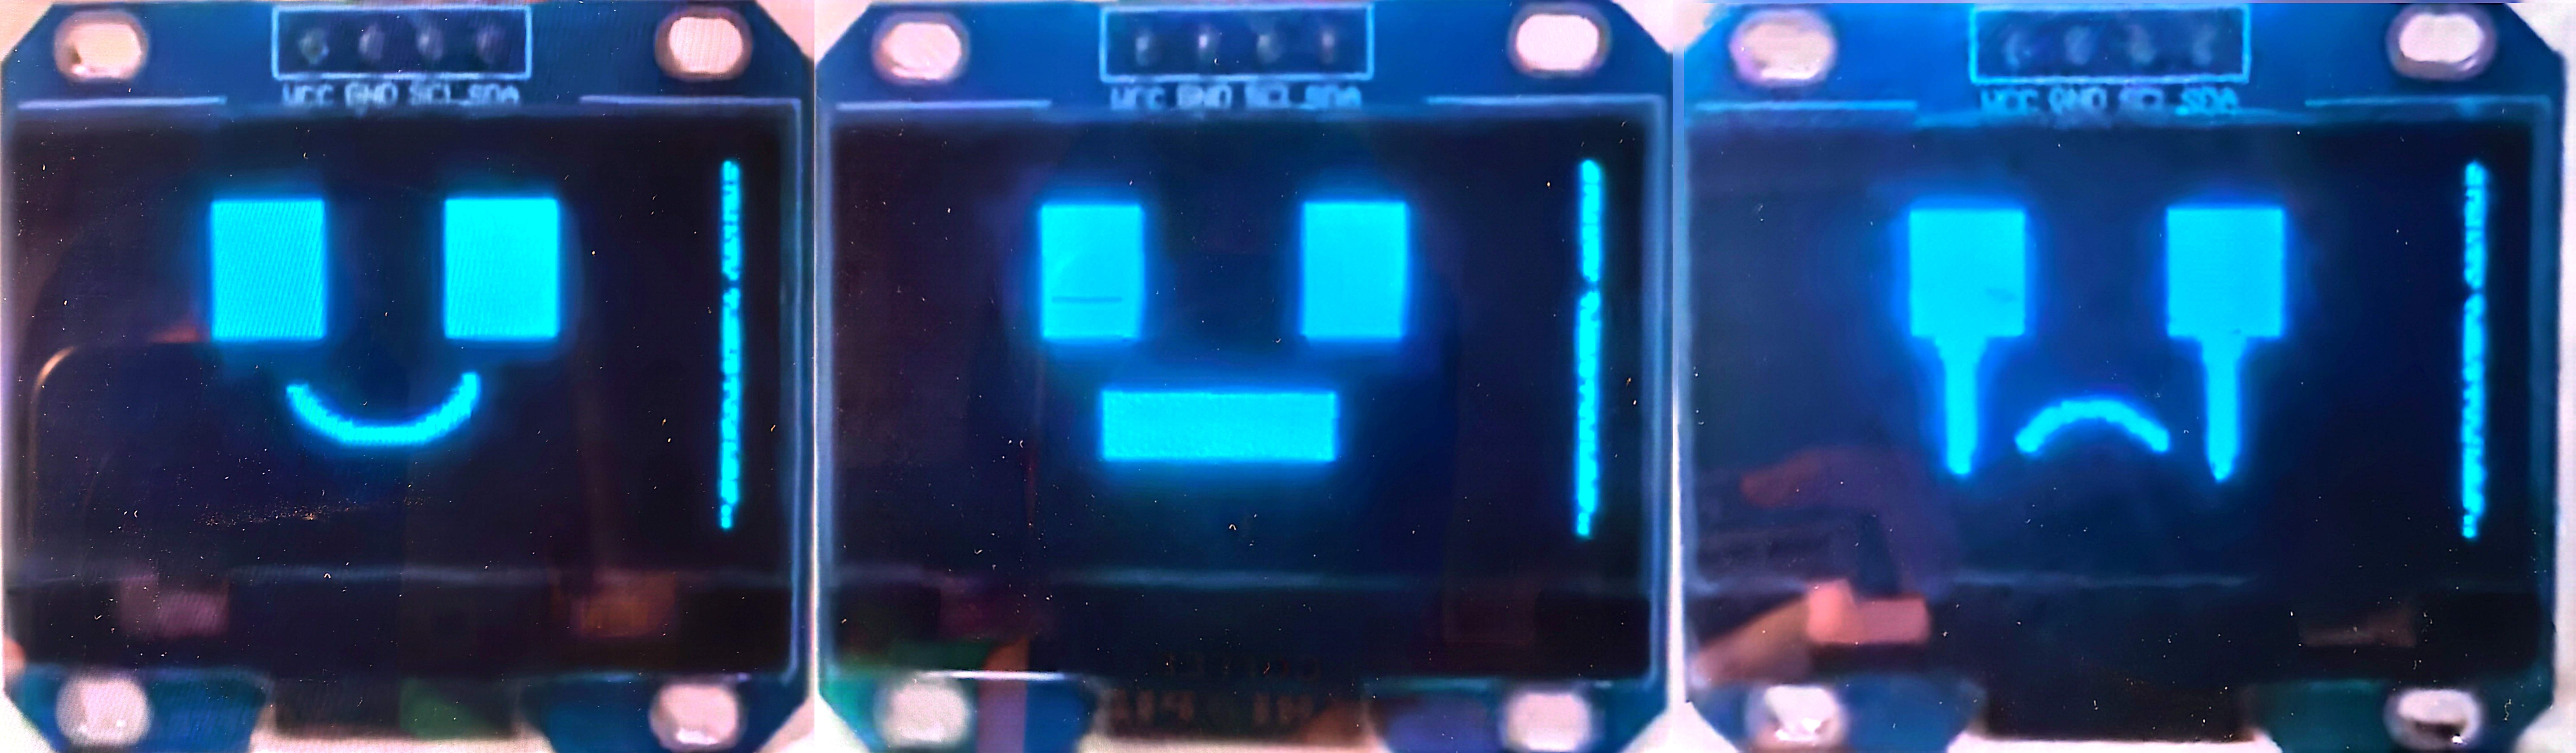
\includegraphics[width=0.8\textwidth]{images/小车表情.jpg} 
    \caption{oled表情显示} 
    \label{fig:表情}
\end{figure}

    \item \textbf{语音情感识别功能}：手机/语音采集端通过语音识别算法，采集用户语音信号，提取语音特征并识别情感类型（开心、平静、难过、生气），将情感结果转化为数字控制指令，通过无线通信模块发送至小车FPGA主控单元。
\end{enumerate}

我们基本实现了开题答辩中的目标，唯一的改变是因为ASR的识别精度问题我们将语音模块从可以识别任意语音的大模型换成了只能识别特定语句的本地部署的识别模块。进一步的，我们完成了差异化动作设计（转圈，前后移动）。

\subsubsection*{上电启动流程}

\begin{enumerate}
    \item FPGA加载配置比特流，所有寄存器复位。
    \item OLED 统经历约500ms上电延时后，自动发送SSD1306初始化命令。
    \item 初始化完成后，OLED显示默认模式对应的表情（平静脸）。
    \item 小车默认进入FOLLOW模式，超声波测距FSM开始循环测量。
    \item PID控制器在每个测量周期结束时更新一次输出，驱动电机完成跟随控制。
\end{enumerate}

\subsubsection*{跟随模式主循环}

\begin{enumerate}
    \item 触发左侧超声波传感器（10$\mu$s脉冲）。
    \item 等待并测量左侧回波时间，存储left\_cnt。
    \item 触发右侧超声波传感器（10$\mu$s脉冲）。
    \item 等待并测量右侧回波时间，存储right\_cnt。
    \item 计算avg\_cnt=(left\_cnt+right\_cnt)$\gg$ 2和 diff\_signed=right\_cnt$-$left\_cnt。
    \item PID速度环根据avg\_cnt输出speed\_ctrl；转向环根据diff\_signed输出turn\_ctrl。
    \item 差速混控：left\_duty=speed\_ctrl + turn\_ctrl，right\_duty = speed\_ctrl $-$ turn\_ctrl。
    \item 更新PWM和IN1/IN2方向信号。
    \item 等待约50ms，进入下一轮测量。
\end{enumerate}

\subsection{设计的课程知识运用}
\subsubsection{运控模块：}
\begin{enumerate}
    \item 运动状态的切换运用了FSM的框架，为了保证小车的基本功能正确运行，我们设置happy状态与sad状态执行完成后均无条件进入neutral状态，使小车“始终”以跟随为主要动作。
    \item 电机驱动逻辑运用组合逻辑，在verilog中体现为条件分支的行为级描述，电机接线依据桥式电路原理。
\end{enumerate}

\subsubsection{表情控制：}
\begin{enumerate}
    \item FSM的工程化应用，顶层采用标准三段式架构，构建 Idle→Init→Clear→On→Show 的完整工作流程，严格遵循数字系统 "初始化 - 等待 - 执行 - 返回" 的经典控制流设计模式；
    \item IIC 串行通信协议的实践，运用 IIC 协议实现 FPGA 与 OLED 显示屏的通讯，完整实现两线式主从通信、双向三态总线控制、字节传输应答等协议核心机制；
    \item 模块化设计思想，将系统拆分为 IIC 主机、初始化、清屏、显示控制等独立功能模块。
\end{enumerate}


\subsection{设计的复杂性}
我们的设计在结构和逻辑上具有一定的复杂性，主要体现在以下几个方面：
\begin{itemize}
    \item \textbf{结构复杂度}：小车的核心组成是三大模块：语音模块，运控模块和表情模块，三个模块协同工作看似耦合复杂，但我们通过“情绪标签”的设计规避了复杂的系统设计，让简单的2-bit数据通过组合逻辑得到稳定的电路控制效果。
    \item \textbf{逻辑复杂度}：由于三个模块的并行机制，每个模块都采用了分支逻辑，happy,sad,neutral3种状态（算上待机/关机是4种）一一对应，控制流分支数量较少，逻辑复杂度低。
    \item \textbf{认知复杂度}：我们的设计思路明确，代码中包括了关键注释，模块所采用的基本都是标准做法（运控模块的控制方式，OLED的驱动模式）并且特意避开了复杂的状态设计，力图用简单的方式实现核心功能。
\end{itemize}

\subsection{设计特点与创新}

\begin{itemize}
    \item \textbf{异构计算架构的协同运行}：不同于传统的单一微处理器方案，我们计划采用两个FPGA和语音模块芯片协同的异构架构，他们共用部分信号输入，同时也有各自专控的部分
    \item \textbf{多模态情感映射}：项目不仅停留在“对话”层面，更创新性地引入了语义情感分析。小车可将抽象情绪（喜、怒、哀、乐）实时映射为三位一体的反馈：视觉（OLED 表情）、听觉（语音回复）及物理动作（旋转、靠近、前后运动）。这种“行为语言”极大增强了陪伴的拟人化程度。
\end{itemize}


% ###########################################################################
% 第五节：总结
% ###########################################################################
\section{总结}

\subsection{设计完成情况}

我们小组的项目成功实现了一台基于FPGA驱动的智能陪伴小车，完成了全部开题时预定的设计目标：

\begin{enumerate}[label=(\arabic*)]
    \item \textbf{控制算法实现}：设计并实现了可参数化的双环PID差速控制算法，能够在理想环境下实现平滑的距离跟随。
    \item \textbf{传感器接口设计}：完成了完整的双路超声波HC-SR04 测距有限状态机，包含两级寄存器异步信号同步、边沿检测和超时保护等鲁棒性设计，确保系统在传感器异常时不会死锁。
    \item \textbf{通信协议实现}：实现了一个完整的I2C Master 控制器，成功驱动SSD1306 OLED屏幕。
    \item \textbf{人机交互设计}：通过语音实现模式转换，OLED屏幕实时反馈对应的情感状态，将功能性控制与情感化表达有机结合。
    \item \textbf{电机驱动设计}：输出了完整的PWM+IN1/IN2方向信号，适配标准L298N H桥驱动模块，支持两路电机的独立正反转。
\end{enumerate}



\subsection{不足与展望}
我们组的问题主要来自硬件的局限性，具体如下：
\begin{enumerate}[label=(\arabic*)]
    \item \textbf{小车在各种环境跑不了问题}：可以优化小车电机，换功率更大的。
    \item \textbf{可变速度未实现}：因为我们的小车电压转换不够，占空比控速未能实现，导致转弯较为不灵敏，和上面一样是硬件优化问题。
    \item \textbf{OLED显示不稳定问题}：如果换用7脚的oled和有稳定的电压输入，显示会更稳定。
    \item \textbf{语音识别模块的局限性}：由于ASRPRO芯片只能识别预设的命令词，无法实现开放式对话。可以考虑在原来已经实现的云端返回对话内容的基础上提高识别灵敏度，用云端LLM模型来实现更自然的语音交互。
    \item \textbf{多模态情感映射的扩展}：目前系统仅支持三种情绪状态（开心、平静、难过），未来可以通过增加更多的情绪类别和对应的动作/表情组合，提升小车的情感表达能力。  
    \item \textbf{状态可视化的增加}：在调试oled以及运控的过程中我们发现我们很难判断我们的小车目前处于什么状态，未来可以增加一个状态显示模块，引入FPGA上的数码管或者led，用于显示当前小车的模式等信息，方便调试。
\end{enumerate}

\subsection{心得}
本次基于FPGA的智能陪伴小车的项目，我们从最初的架构到最终的实物稳定运行，整个开发过程带给我们诸多超越课本知识的启示与深刻体会。

在项目开发过程中，我们体会到了Verilog和FPGA的应用。与传统MCU的串行轮询不同，FPGA允许双路测距、PID 算法、I2C协议栈独立并行运转。这种硬件级别的实时响应，保证了系统较快的联动反馈，感受到了并行设计思维。在各个模块的优化迭代中，我们也深刻理解了模块化设计、状态机设计和通信协议实现的实际应用价值，以及多路径实现的可能性。

无疑，此次课程设计为日后的科研以及工程训练打下坚实的基础。我们不仅掌握了FPGA的开发流程，还在实践中锻炼了团队协作、问题分析和解决能力。通过不断调试和优化，我们学会了如何在有限的硬件资源下实现复杂功能，并对系统设计有了更全面的理解。
% ###########################################################################
% 附录
% ###########################################################################
\appendix

\section{代码结构}
\subsection{模块结构}

系统的完整模块依赖关系如图~\ref{fig:full_deps} 所示。箭头方向表示"被调用"关系（即上层模块实例化下层模块）。

\begin{figure}[H]
\centering
\begin{tikzpicture}[
    node distance=0.5cm,
    module/.style={rectangle, draw, minimum width=3cm, minimum height=0.7cm, align=center, font=\footnotesize},
    arrow/.style={->, >=stealth}
]

% 主控侧
\node[module, fill=blue!10] (ctrl) {control.v};
\node[module, below=0.3cm of ctrl] (pidL) {pid\_controller（速度环）};
\node[module, below=0.3cm of pidL] (pidR) {pid\_controller（转向环）};

% OLED 侧
\node[module, fill=blue!10, right=2.5cm of ctrl] (top) {topcontrol.v};
\node[module, below=0.3cm of top] (oledtop) {Oled\_Top.v};
\node[module, below=0.3cm of oledtop] (i2c) {iic.v（I2C Master）};

% OLED 功能模块
\node[module, below=0.8cm of i2c, xshift=-1.8cm] (init) {Oled\_Init.v};
\node[module, right=0.5cm of init] (clear) {Oled\_Clear.v};
\node[module, right=0.5cm of clear] (on) {Oled\_On.v};
\node[module, below=0.5cm of init, xshift=1.3cm] (showctl) {Oled\_Show\_control.v};
\node[module, below=0.5cm of showctl] (showinfo) {Oled\_Show\_Info.v};
\node[module, below=0.5cm of showinfo] (font) {font\_data.v};

% 连线
\draw[arrow] (ctrl) -- (pidL);
\draw[arrow] (pidL) -- (pidR);
\draw[arrow] (top) -- (oledtop);
\draw[arrow] (oledtop) -- (i2c);
\draw[arrow] (i2c.south) -- ++(0,-0.3) -| (init.north);
\draw[arrow] (i2c.south) -- ++(0,-0.3) -| (clear.north);
\draw[arrow] (i2c.south) -- ++(0,-0.3) -| (on.north);
\draw[arrow] (i2c.south) -- ++(0,-0.3) -| (showctl.north);
\draw[arrow] (showctl) -- (showinfo);
\draw[arrow] (showinfo) -- (font);

% OLED 功能模块虚线框
\node[draw, dashed, fit=(init)(clear)(on)(showctl)(showinfo)(font), inner sep=4pt, label={[font=\footnotesize]below:OLED 显示功能模块}] {};

\end{tikzpicture}
\caption{系统模块依赖关系图}
\label{fig:full_deps}
\end{figure}




% ###########################################################################
% 附录：完整代码
% ###########################################################################
\section{完整代码}

\subsection{control.v}

\lstinputlisting[caption={control.v —— 主控模块（PID + 超声波测距 + 电机控制）}]{../control.v}

\subsection{OLED/iic.v}

\lstinputlisting[caption={iic.v —— I2C Master 通信协议}]{../OLED/iic.v}

\subsection{OLED/font\_data.v}

\lstinputlisting[caption={font\_data.v —— 16×16 表情字模数据}]{../OLED/font_data.v}

\subsection{OLED/Oled\_Top.v}

\lstinputlisting[caption={Oled\_Top.v —— OLED 顶层调度状态机}]{../OLED/Oled_Top.v}

\subsection{OLED/Oled\_Init.v}

\lstinputlisting[caption={Oled\_Init.v —— SSD1306 初始化配置}]{../OLED/Oled_Init.v}

\subsection{OLED/Oled\_Show\_control.v}

\lstinputlisting[caption={Oled\_Show\_control.v —— 显示坐标定位}]{../OLED/Oled_Show_control.v}

\subsection{OLED/Oled\_Show\_Info.v}

\lstinputlisting[caption={Oled\_Show\_Info.v —— 显示信息输出}]{../OLED/Oled_Show_Info.v}

\subsection{OLED/Oled\_Clear.v}

\lstinputlisting[caption={Oled\_Clear.v —— 全屏清除控制}]{../OLED/Oled_Clear.v}

\subsection{OLED/Oled\_On.v}

\lstinputlisting[caption={Oled\_On.v—— 全屏点亮控制}]{../OLED/Oled_On.v}

\subsection{OLED/topcontrol.v}

\lstinputlisting[caption={topcontrol.v —— OLED 顶层封装（SW 检测与自动复位）}]{../OLED/topcontrol.v}

\end{document}
